\everymath{\displaystyle}
\usepgfplotslibrary{fillbetween}

%%%%%%%%%%%%%%%%%%%%%%%%%%%%%%%%%%%%%%%%
%           main body
%%%%%%%%%%%%%%%%%%%%%%%%%%%%%%%%%%%%%%%%

%-----------------------------------
%	TITLE PAGE
%-----------------------------------

\title[第七章\\
定积分]{\texorpdfstring{\LARGE \bfseries 第七章\quad 定积分}{第七章 定积分}} % The short title appears at the bottom of every slide, the full title is only on the title page
\author[\smaller \S 7.4\\
几何计算中的应用] % Your institution as it will appear on the bottom of every slide, maybe shorthand to save space
{\Large \bfseries \S 7.4 定积分在几何计算中的应用}
% \author{Singular Value Decomposition} % Your name
% \date{\today} % Date, can be changed to a custom date
\date{}

%------------------------------------------------

\begin{document}

%------------------------------------------------

\begin{frame}

\titlepage % Print the title page as the first slide

\end{frame}

%------------------------------------------------

% \begin{frame}
% \frametitle{内容提要} % Table of contents slide, comment this block out to remove it
% \tableofcontents % Throughout your presentation, if you choose to use \section{} and \subsection{} commands, these will automatically be printed on this slide as an overview of your presentation
% \end{frame}

%-----------------------------------
%	PRESENTATION SLIDES
%-----------------------------------

%------------------------------------------------

\begin{frame}
\frametitle{绪言}

{
\larger[2]

正如这章引入定积分概念时所说, 定积分可以用来求一些``不规则''曲线长度, 曲面面积, 以及某些立体的体积等几何量, 以及一些物理问题 (下一节).

}

\end{frame}

%------------------------------------------------

\section{平面图形面积}

%------------------------------------------------

\begin{frame}
\frametitle{平面图形面积 -- 问题的引入}

\begin{recall}[定积分定义]
由 $f(x)$ 给出的曲线 $y=f(x)$ 与 $x$ 轴 ($y = 0$), 以及两条竖直线 $x=a$ 和 $x=b$ 围成的图形的\alert{带符号}面积为
\[
\text{面积} = \int_a^b f(x) ~ dx.
\]
\end{recall}

\pause

更一般地, $x$ 轴可以替换为另一条曲线 $y=g(x)$, 这时由 $f(x)$, $g(x)$; $x=a$ 和 $x=b$ (有时隐含) 围成的图形的带符号面积为
\[
\text{面积} = \int_a^b [f(x) - g(x)] ~ dx = \int_a^b f(x) ~ dx - \int_a^b g(x) ~ dx.
\]

\pause

\textbf{求解要点:} 把图形画出来, 将问题表达为一个定积分, 计算定积分.

\end{frame}

%------------------------------------------------

\begin{frame}
\frametitle{平面图形面积 -- 例题}

\begin{eg}
求曲线 $y = x^2$ 与 $x = y^2$ 围成的区域的面积.
\end{eg}

\pause

\begin{columns}
\begin{column}{0.35\textwidth}
\begin{center}
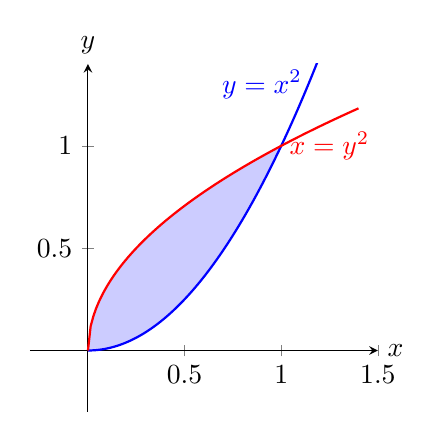
\begin{tikzpicture}
\begin{axis}[
    axis lines=middle,
    xlabel={$x$},
    ylabel={$y$},
    xlabel style={at={(ticklabel* cs:1)}, anchor=west},
    ylabel style={at={(ticklabel* cs:1)}, anchor=south},
    xmin=-0.3, xmax=1.5,
    ymin=-0.3, ymax=1.4,
    domain=0:1.2,
    samples=100,
    width=6cm,
    height=6cm,
]

% 绘制曲线 y = x^2
\addplot[blue, thick, domain=0:1.2, name path=A] {x^2};
\node[blue] at (axis cs:0.9,1.3) {$y=x^2$};

% 绘制曲线 x = y^2 (即 y = sqrt(x))
\addplot[red, thick, domain=0:1.4, name path=B] {sqrt(x)};
\node[red] at (axis cs:1.25,1.0) {$x=y^2$};

% 填充两条曲线之间的区域
\addplot[fill=blue!20] fill between[of=A and B, soft clip={domain=0:1}];

\end{axis}
\end{tikzpicture}
\end{center}
\end{column}
\begin{column}{0.65\textwidth}
\textbf{解:} 联立方程 $y = x^2$ 和 $x = y^2$ 可得交点为 $(0,0)$ 和 $(1,1)$. 由图可知, 在 $x \in [0,1]$ 上, 曲线 $y = x^2$ 在上方, 曲线 $x = y^2$ 在下方. 因此, 所求面积为
\[
\int_0^1 (x^2 - \sqrt{x}) ~ dx = \int_0^1 x^2 ~ dx - \int_0^1 \sqrt{x} ~ dx = \frac{1}{3} - \frac{2}{3} = -\frac{1}{3}.
\]
\end{column}
\end{columns}

\end{frame}

%------------------------------------------------

\begin{frame}
\frametitle{平面图形面积 -- 例题}

\begin{eg}[双曲函数]
求双曲线 $x^2 - y^2 = 1$ 与 $OA = (x_0, y_0)$, $OB = (x_0, -y_0)$ 围成的区域的面积
\end{eg}

\begin{columns}
\begin{column}{0.35\textwidth}
\begin{center}
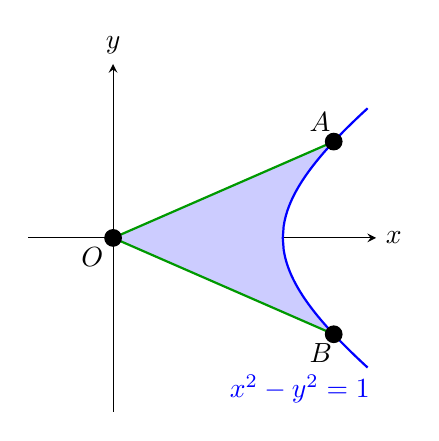
\begin{tikzpicture}
\begin{axis}[
    axis lines=middle,
    xlabel={$x$},
    ylabel={$y$},
    xlabel style={at={(ticklabel* cs:1)}, anchor=west},
    ylabel style={at={(ticklabel* cs:1)}, anchor=south},
    xmin=-0.5, xmax=1.55,
    ymin=-1.5, ymax=1.5,
    samples=100,
    width=6cm,
    height=6cm,
    xtick=\empty,  % 去掉x轴ticks
    ytick=\empty,  % 去掉y轴ticks
]
% 设定点A的坐标
\def\xa{1.3}
\pgfmathsetmacro{\ya}{sqrt(\xa*\xa-1)}

% 绘制填充区域
\addplot[fill=blue!20, draw=none] coordinates {(0,0) (\xa,\ya)} -- plot[domain=\xa:1, samples=50] (\x, {sqrt(\x*\x-1)}) -- (1,0) -- (0,0);
\addplot[fill=blue!20, draw=none] coordinates {(0,0) (\xa,-\ya)} -- plot[domain=\xa:1, samples=50] (\x, {-sqrt(\x*\x-1)}) -- (1,0) -- (0,0);

% 绘制双曲线右支
\addplot[blue, thick, domain=1:1.5, name path=upper] {sqrt(x^2-1)};
\addplot[blue, thick, domain=1:1.5, name path=lower] {-sqrt(x^2-1)};

% 绘制线段OA和OB
\addplot[green!60!black, thick] coordinates {(0,0) (\xa,\ya)};
\addplot[green!60!black, thick] coordinates {(0,0) (\xa,-\ya)};

% 标记点
\addplot[only marks, mark=*, mark size=3pt] coordinates {(0,0) (\xa,\ya) (\xa,-\ya)};

% 标签
\node[below left] at (axis cs:0,0) {$O$};
\node[above right] at (axis cs:\xa-0.2,\ya) {$A$};
\node[below right] at (axis cs:\xa-0.2,-\ya) {$B$};
\node[blue] at (axis cs:1.1,-1.3) {$x^2-y^2=1$};
\end{axis}
\end{tikzpicture}
\end{center}
\end{column}
\pause
\begin{column}{0.65\textwidth}
\textbf{解:} 若以 $x$ 为自变量, 则 $y = \pm \sqrt{x^2 - 1}$. 因此, 利用对称性, 所求面积为
\[
\text{面积} = 2 \left( \frac{x_0y_0}{2} - \int_1^{x_0} \sqrt{x^2 - 1} ~ dx \right) = \ln (x_0 + y_0).
\]
注意, 以上是求三角形 $OAB$ 内补面积的方式进行求解.
\pause
也可以以 $y$ 为自变量, 则 $x = \sqrt{y^2 + 1}$. 因此, 利用对称性, 所求面积为
\[
\text{面积} = 2 \left( \int_0^{y_0} \left( \sqrt{y^2 + 1} - \frac{x_0}{y_0} y \right) ~ dy \right) = \ln (x_0 + y_0).
\]
\end{column}
\end{columns}

\end{frame}

%------------------------------------------------

\section{极坐标下求面积}

%------------------------------------------------

\begin{frame}
\frametitle{极坐标下求面积问题的引入}

\end{frame}

%------------------------------------------------

\section{旋转体体积}

%------------------------------------------------

\begin{frame}
\frametitle{旋转体体积}

\end{frame}

%------------------------------------------------

\end{document}
